Lors des différentes expériences effectuées, notamment sur les cas d'échec de convergence, une observation à priori étonnante a pu être faite sur l'impact de la valeur des paramètres de contrôle $\alpha$ (ou $p$), notamment celui de leur signe, sur la direction dans laquelle converge le réseau lors de son entraînement. Les couches morphologiques, en particulier $\mathcal{S}$Morph et $\mathcal{S}$MorphTanh, se comportent en effet comme des moyenneurs quand leur paramètre de contrôle $\alpha$ est proche de 0, peu importe son signe. On pouvait alors espérer que la différence de comportement d'un réseau, dont le paramètre $\alpha$ d'une couche est proche de 0, serait minime voire négligeable entre un $\alpha$ positif et un $\alpha$ négatif. Or, plusieurs expériences permettent de montrer que le signe des paramètres $\alpha$, même très proches de 0, a un impact majeur, voire plus important que la forme des noyaux $w$, sur la direction de convergence des réseaux. \\

%figure
\vspace{-0.6mm}
\begin{figure}[htp]
  \begin{center}
    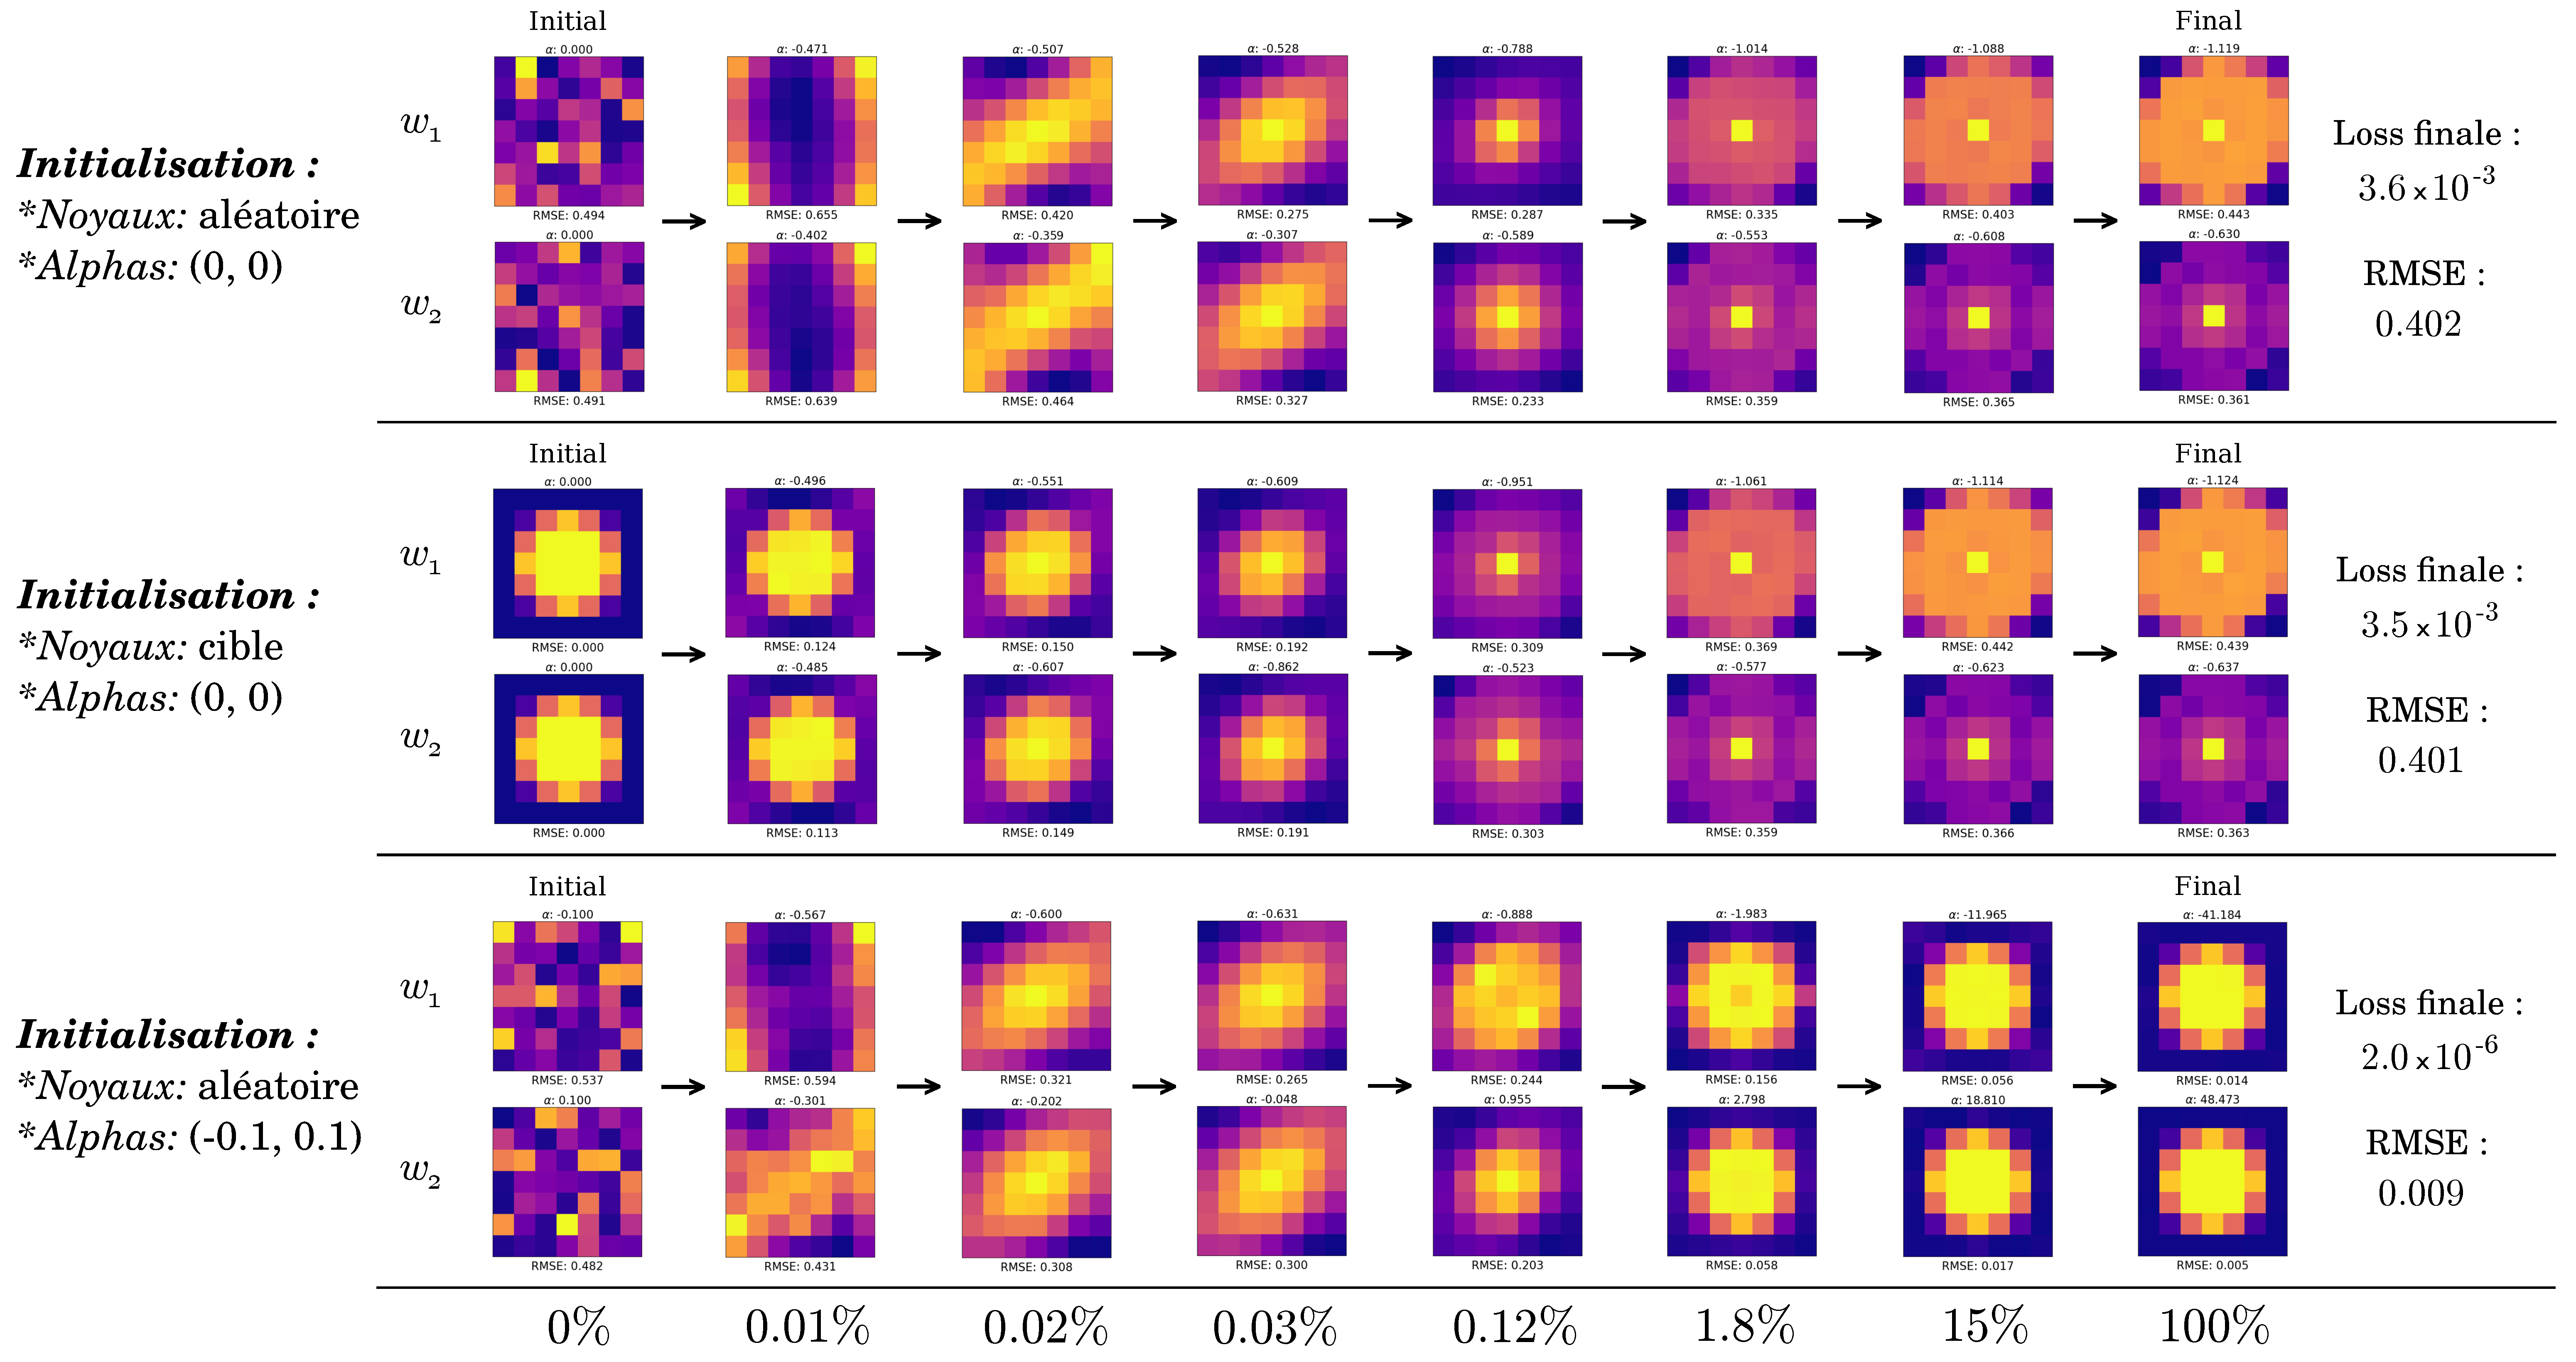
\includegraphics[width=1.00\linewidth]{parts/4-analyse_des_reseaux/others/figures/zzzzz.pdf}
    \vspace{-4.0mm}
    \caption{ \centering Évolution de la forme des deux noyaux $w$ du réseau $\mathcal{S}$MorphNetTanh et de leur \textit{RMSE} en fonction de la progression de l'entraînement (en \% avant l'état final), pour l'ouverture sur MNIST avec le \textit{disk2}, sur trois types d'initialisation.}
    \label{fig:zzzzz}
  \end{center}
\end{figure}

\vspace{-2.0mm}
%La figure \ref{fig:zzzzz} ci-dessus montre en effet, sur un cas où le réseau $\mathcal{S}$MorphNetTanh à deux couches sans contrainte, avec l'opération cible d'ouverture et la structure cible \textit{disk2} sur MNIST, converge initialement vers un échec (tiers haut), que ce même réseau, en initialisant ses noyaux avec la structure cible exacte, converge exactement vers le même état d'échec (tiers milieu), mais que ce réseau encore, avec cette fois uniquement une initialisation des paramètres de contrôle $\alpha$ de très faible amplitude (0.1) mais du signe recherché, converge effectivement bien vers l'état cible de succès (tiers bas).
La figure \ref{fig:zzzzz} ci-dessus illustre le cas du réseau $\mathcal{S}$MorphNetTanh à deux couches morphologiques - muni d'aucune contrainte sur ces dernières ni d'aucun partage de poids, dont l'opération cible est l'ouverture et la structure cible est le \textit{disk2}, et entraîné sur MNIST -, qui converge initialement vers un échec (tiers supérieur de la figure).

\newpage

\noindent Ce même réseau, en initialisant ses deux noyaux par la structure cible exacte recherchée, converge exactement vers le même état d'échec (tiers central). Cependant, ce même réseau encore, avec cette fois uniquement une initialisation des paramètres de contrôle $\alpha$ de très faible amplitude ($|\alpha| = 0.1$) mais du signe recherché (négatif pour $\alpha_1$ et positif pour $\alpha_2$, comme on est dans le cadre d'une opération cible d'ouverture), converge effectivement bien vers l'état cible de succès (tiers inférieur). \\

\vspace{-1.6mm}
%\noindent 
Cela montre que le déplacement des paramètres de contrôle $\alpha$, même de très faible amplitude, vers leur signe cible respectif, a un impact bien plus important sur la réussite de la convergence que ne l'a le déplacement des poids des noyaux vers la forme exacte de la structure cible. Cette même conclusion peut être faite sur d'autres expériences encore qui sont initialement des échecs, et dont le signe des $\alpha$ dans leur état final n'est pas le bon recherché. Une bonne valeur (à l'initialisation ou au cours de l'entraînement) des paramètres de contrôle $\alpha$, et en particulier le bon signe de ces paramètres, a donc une importance majeure, probablement supérieure à celle de la forme des noyaux $w$, dans le succès de la convergence des réseaux.

\vspace{1.0mm}


%Importance des paramètres de contrôle $\alpha$ des couches morphologiques dans la convergence des réseaux
%+ Parler de l'impact des alphas sur la convergence des réseaux : pour certains échecs où les deux $\alpha$ finissent par être proches de 0 et du même signe, l'initialisation des noyaux $w$ en la forme cible n'est même pas suffisante pour que le réseau converge bien. Par contre, l'initialisation des $\alpha$ avec le bon signe pour chacun et une très faible amplitude, tout en gardant une forme aléatoire pour l'initalisation des $w$, permet quant à elle de faire converger le réseau corresctement.
